\chapter*{Introduction}
\addcontentsline{toc}{chapter}{Introduction}
One of big unsolved problems of the modern physics is the construction of quantum computer. The implications here are mainly to so-called \emph{adiabatic quantum computers}, where the solution to some mathematical problem is substituted for finding the energy minima in some system of coupled qubits\footnote{As qubits one might use for example quantum dots \citep{dots}, or Josephson junctions \citep{josephson}.}. The energy minima can be found by numerous measurements of the specific superposition of qubits. The preparation of such superposed state is complicated process and one method of achieving it is so-called \emph{quantum annealing}\footnote{The name comes from the resemblance to annealing in metallurgy.}. This is the process of changing the state from some simple \emph{initial state} to the required state in superposition (\emph{final state}). The initial state is typically chosen to be the ground state of some easily obtainable configuration, such as \emph{all spins up}. The change in states is called \emph{quantum state transport} or \emph{quantum state driving}.

The point of interest of this thesis is the quantum state driving. This driving usually needs to be performed \emph{adiabatically}, i.e., without excitation of the system. The probability that the state will remain in a ground state during such transport is called \emph{fidelity}. For illustration of this problem see Fig. \ref{fig:introDriving}, where two scenarios are drawn. First, the state moves adiabatically (fidelity is one), second, the state excites in the small energy gap area, which in the case of quantum computers devaluates the experiment.

\begin{figure}[H]
    \centering
    \begin{tikzpicture}
        \node[] at (0,0) {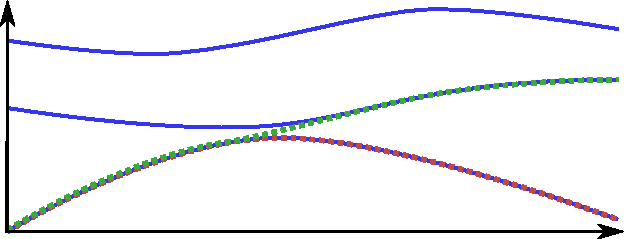
\includegraphics[width=0.6\textwidth]{../img/introDriving.pdf}};
        \node[] at (-4.5,1.6) {$\blue E$};
        \node[] at (4.6,-1.55) {$t$};
    \end{tikzpicture}
\caption{Visualization of the \redd{state adiabatic transport} compared to \greenn{transport with excitation} in a system with time varying \bluee{energy eigenstates}.}
    \label{fig:introDriving}
\end{figure}

This problem is of course more general. From mathematical point of view, in the example above we have \emph{parameter driven Hamiltonian} $\HH(\llambda)$ between qubits (omitting the thermal basis of the environment and other effects), which depends on some vector $\llambda$ from \emph{parameter space}. Change in the driving parameter (for example orientation of a magnetic field, or strength of qubit coupling) influences the qubits and \emph{drives} them to some final state in superposition.

The question of interest is: “How to achieve the better \emph{final fidelity}, meaning \emph{how to prepare the final ground state with the higher probability}?” During the driving one might add some energy to the qubit, which leads to its excitation and possibly destroys the superposition. This can be improved by many methods. From the theory of \emph{quantum state driving} three methods are emphasized here — \emph{adiabatic driving}, \emph{counter-diabatic driving}, or \emph{choosing better driving path}. Adiabatic driving can be performed by infinitely slow drivings, making it unsuitable for practical applications. Counter-diabatic driving requires adding another element to the Hamiltonian, which leads to \emph{unit fidelity protocols} (the system does not excite), making it a good candidate for practical applications. The method of finding better driving path can be combined with all other methods, and means that different paths in parameter space lead to different fidelity. Because these trajectories are influenced by energy spectra, one might be interested in the \emph{quantum state manifolds}. These are especially important for some drivings, such as driving using small \emph{quenches} (quick, but small changes in driving parameter), or close-adiabatic driving, where the fidelity is almost one.

To understand the geometry of quantum state driving, the basics of differential geometry are presented in Chapter \ref{chap:mathIntro}. It does not serve the full theory, only some basic intuition is build and useful definitions are provided here. The theory of quantum driving itself is described in Chapter \ref{chap:driving}. First the geometrical space is constructed, then the concept of \emph{quantum state driving}, \emph{fidelity} and \emph{metric tensor} are introduced.
The driving methods are described in Chapter \ref{chap:typesOfDriving}. Especially \emph{counter-diabatic}, \emph{adiabatic} and \emph{close-adiabatic} drivings are introduced, along with reformulation of theorems about fidelity. Special importance is played by the \emph{ground state manifold} and geodesics, for which some applications are proposed.

To understand the general fidelity driving, a simple two level system is analyzed in Chapter \ref{chap:twoLevelSystem}. Driving fidelity and energy variance are calculated for two special drivings — \emph{linear} and \emph{geodesic}. This demonstrates some basic phenomena which occur in quantum state driving in general. Finally, the more convoluted Lipkin-Meshkov-Glick model is analyzed in Chapter \ref{chap:lipkin}. The analysis is first performed in specific dimensions, from which some general formulas in arbitrary dimension are derived. Focus is especially on the ground state manifold and geometrical structures on it. This can help to understand drivings with unit or almost unit fidelity.